\documentclass[isoft]{ufgposter}

\usepackage{lipsum}
\usepackage{natbib}
\usepackage{booktabs}
\usepackage{subfig} 
\usepackage{amsmath} 
\usepackage{textcomp} 
\usepackage{url}  
\usepackage{hyperref}
\usepackage[utf8]{inputenc}
\usepackage[portuguese]{babel}

%%%%%%%%%%%%%%%%%%%%%%%%%%%%%%%%%%%%%%%%%
%%               Configs               %%
%%%%%%%%%%%%%%%%%%%%%%%%%%%%%%%%%%%%%%%%%

% Choose one of the section color {ufglhblue | ufgdkblue | dkblue | black | gold}
\sectionfont{\color{gold}} 

% Informe complete path to the logo files or leave empty one or both parameter. 
\settinglogos{images/ufg-logo}{images/department-logo}

% Choose one of the backgound options {1 | 2 | 3} 
\setbackground{3}

% General info
\title{\uppercase{NomeDeImpacto: Aqui vai o título \\ com uma quebra de linha no meio}} 
\author{Altino Dantas, Anderson Soares e Celso G. Camilo-Junior Altino Dantas, Anderson Soares e } 
\department{Instituto de Informática - INF}
\site{i4soft.com.br}
\class{Projeto Ciência no Parque}
\posteryear{2018}
\copyrightholder{Intelligence for Software Research Group - i4Soft}

%%%%%%%%%%%%%%%%%%%%%%%%%%%%%%%%%%%%%%%%%
%%           End configs               %%
%%%%%%%%%%%%%%%%%%%%%%%%%%%%%%%%%%%%%%%%%

\pagestyle{fancy}
\begin{document}
\begin{poster}

%%%%%%%%%%%%%%%%%%%%%%%%%%%%%%%%%%%%%%%%%
%%        Begin of the poster          %%
%%%%%%%%%%%%%%%%%%%%%%%%%%%%%%%%%%%%%%%%%

\section{Introdução}

\lipsum[3-4]

\section{Materiais e métodos}%

\subsection{Coloque aqui seu modelo}

\lipsum[11]

\vspace{1cm}

\begin{figure}
\centering
\captionsetup{type=figure}
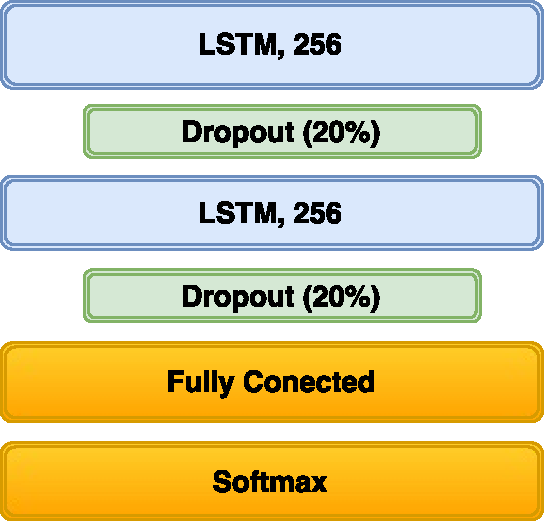
\includegraphics[scale=2]{lstm}
\caption{Arquitetura de rede LSTM utilizado no trabalho.}
\label{fig:lstm}
\end{figure}

\subsection{Coloque aqui seu \textit{dataset}}

\lipsum[54]

\vspace{1cm}
\begin{table}
\centering
\captionsetup{type=table}
\caption{\textit{Corpus} utilizados no estudo}
\label{Corpus}
\renewcommand{\arraystretch}{1.2}
\resizebox{0.47\textwidth}{!}{%
\begin{tabular}{lcccclcl}
\hline
&\textbf{Corpus}    &  \textbf{Caracteres únicos} &    &  \textbf{Total de linhas}  &  & \textbf{Total de caracteres} &  \\ \hline
&SBSEThesis         & 88  &    &    2.311     &        & 771.179 &  \\ 
&Bible              & 63  &    &    32.359   &        & 3.924.374 &  \\
&JavaCode           & 69  &    &    436.565  &        & 12.053.424 &  \\ \hline
\end{tabular}
}
\end{table}
\vspace{1cm}

\lipsum[57]

\citep{defects2j}.

\subsection{Subsection}
\lipsum[8]

\section{Resultados}%

\begin{figure}
\centering
\captionsetup{type=figure}
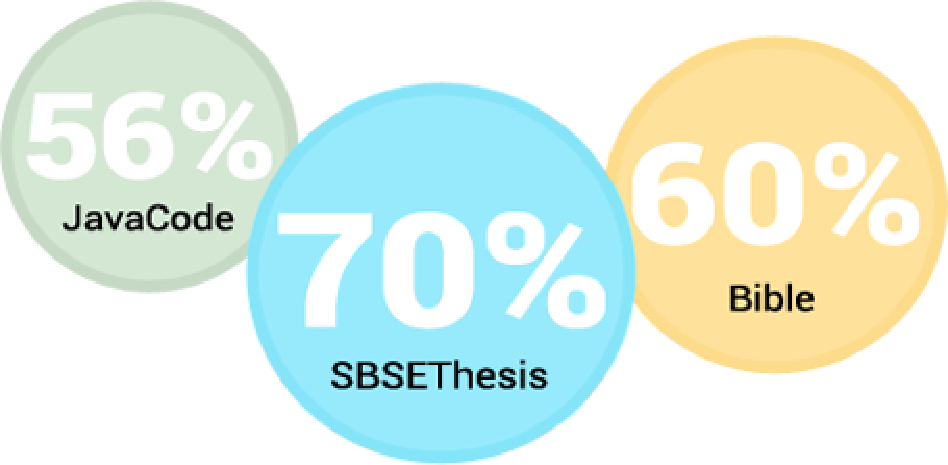
\includegraphics[scale=2]{resultado}
\caption{Taxa de sucesso de predição por \textit{corpus}.}
\label{fig:result}
\end{figure}

\lipsum[5]
\cite{chollet2015keras}

\section{Considerações finais}

\lipsum[15]

\section{Agradecimento}

\lipsum[57]

\bibliographystyle{abbrv}
\bibliography{refs}

%%%%%%%%%%%%%%%%%%%%%%%%%%%%%%%%%%%%%%%%%
%%          End of the poster          %%
%%%%%%%%%%%%%%%%%%%%%%%%%%%%%%%%%%%%%%%%%

\end{poster}

\end{document}

 
